% ============================================================
%  DISCOVERY CURRICULUM — Journey 4, Module 3
%  "The Classical PDEs"
%  Compile with: pdflatex J4_M3.tex  (run twice)
% ============================================================
\documentclass[12pt,a4paper]{article}
\usepackage[a4paper,top=2.5cm,bottom=2.5cm,left=2.8cm,right=2.8cm,headheight=15pt]{geometry}
\usepackage{amsmath,amssymb,amsthm}
\usepackage{xcolor}
\usepackage{mdframed}
\usepackage{enumitem}
\usepackage{tikz}
\usetikzlibrary{arrows.meta,calc}
\usepackage{pgfplots}
\pgfplotsset{compat=1.18}
\usepackage{booktabs}
\usepackage{fancyhdr}
\usepackage{titlesec}
\usepackage{parskip}
\usepackage{hyperref}
\hypersetup{colorlinks=true,linkcolor=NavyBlue,urlcolor=NavyBlue}

\definecolor{NavyBlue}{HTML}{1A3A5C}
\definecolor{MidBlue}{HTML}{2E6DA4}
\definecolor{Gold}{HTML}{C8922A}
\definecolor{LightBlue}{HTML}{EBF2FA}
\definecolor{LightGold}{HTML}{FDF4E3}
\definecolor{DarkGrey}{HTML}{3A3A3A}
\definecolor{BoxGreen}{HTML}{E8F5E9}
\definecolor{SidebarGrey}{HTML}{F5F5F5}

\titleformat{\section}{\Large\bfseries\color{NavyBlue}}{}{0em}{}[{\color{MidBlue}\vspace{2pt}\rule{\linewidth}{1.5pt}}]
\titleformat{\subsection}{\large\bfseries\color{MidBlue}}{}{0em}{}

\pagestyle{fancy}\fancyhf{}
\fancyhead[L]{\small\color{DarkGrey}\textit{Discovery Curriculum}}
\fancyhead[R]{\small\color{DarkGrey}\textit{Journey 4 $\cdot$ Module 3}}
\fancyfoot[C]{\small\color{MidBlue}\thepage}
\renewcommand{\headrulewidth}{0.4pt}

\newmdenv[backgroundcolor=NavyBlue!7,linecolor=NavyBlue,linewidth=2pt,leftline=true,rightline=false,topline=false,bottomline=false,innerleftmargin=14pt,innerrightmargin=10pt,innertopmargin=10pt,innerbottommargin=10pt,skipabove=14pt,skipbelow=10pt]{puzzlebox}
\newmdenv[backgroundcolor=LightGold,linecolor=Gold,linewidth=2pt,leftline=true,rightline=false,topline=false,bottomline=false,innerleftmargin=14pt,innerrightmargin=10pt,innertopmargin=10pt,innerbottommargin=10pt,skipabove=14pt,skipbelow=10pt]{discoverybox}
\newmdenv[backgroundcolor=LightBlue,linecolor=MidBlue,linewidth=1.5pt,roundcorner=4pt,innerleftmargin=14pt,innerrightmargin=10pt,innertopmargin=10pt,innerbottommargin=10pt,skipabove=14pt,skipbelow=10pt]{namebox}
\newmdenv[backgroundcolor=BoxGreen,linecolor=DarkGrey!35,linewidth=1pt,roundcorner=4pt,innerleftmargin=14pt,innerrightmargin=10pt,innertopmargin=10pt,innerbottommargin=10pt,skipabove=14pt,skipbelow=10pt]{reflectionbox}
\newmdenv[backgroundcolor=SidebarGrey,linecolor=Gold,linewidth=1.2pt,leftline=true,rightline=false,topline=false,bottomline=false,innerleftmargin=12pt,innerrightmargin=10pt,innertopmargin=7pt,innerbottommargin=7pt,skipabove=10pt,skipbelow=10pt]{thought}

\newcounter{problem}
\newenvironment{problem}[1][]{\refstepcounter{problem}\par\vspace{6pt}\noindent\textbf{\color{MidBlue}Problem \theproblem}\ifx&#1&\else\ \textit{(#1)}\fi\textbf{.}\enskip}{\par\vspace{4pt}}
\newcounter{deepproblem}
\newenvironment{deepproblem}[1][]{\refstepcounter{deepproblem}\par\vspace{6pt}\noindent\textbf{\color{NavyBlue}$\bigstar$\ Deep Problem \thedeepproblem}\ifx&#1&\else\ \textit{(#1)}\fi\textbf{.}\enskip}{\par\vspace{4pt}}

\begin{document}

\thispagestyle{empty}
\begin{center}
{\small\color{MidBlue}\textbf{DISCOVERY CURRICULUM}\quad$\cdot$\quad\textbf{JOURNEY 4: FIELDS AND SPACE}}
\vspace{0.6cm}

{\color{NavyBlue}\rule{\linewidth}{2pt}}\vspace{0.5cm}

{\Huge\bfseries\color{NavyBlue}Module 3}\\[0.3cm]
{\LARGE\bfseries\color{MidBlue}The Classical PDEs}\\[0.4cm]
{\color{Gold}\rule{0.4\linewidth}{1.2pt}}\\[0.4cm]
{\large\itshape\color{DarkGrey}
Three equations. Electrostatics, heat, waves.\\[0.15cm]
The same operator --- $\nabla^2$ --- governs all three.}

\vspace{1cm}
\begin{tabular}{rl}
\color{DarkGrey}\textbf{Journey}         & Journey 4 --- Fields and Space \\[4pt]
\color{DarkGrey}\textbf{Module}          & 3 of 6 \\[4pt]
\color{DarkGrey}\textbf{Prerequisites}   & J4 Modules 1--2; J2 Module 5; J3 Modules 3, 6 \\[4pt]
\color{DarkGrey}\textbf{You will discover} & Laplace, heat, and wave equations; separation of variables; d'Alembert; Green's functions \\[4pt]
\color{DarkGrey}\textbf{Format}          & 8 problems $+$ 3 deep problems $\approx$ 15 pages \\
\end{tabular}
\vspace{1cm}

{\color{NavyBlue}\rule{\linewidth}{2pt}}
\end{center}

\vspace{0.5cm}
\noindent\textbf{The three equations.}
Classical physics is governed by three partial differential equations involving the Laplacian $\nabla^2$:
\[
  \nabla^2 u = 0 \quad\text{(Laplace)}, \qquad
  \partial_t u = \kappa\nabla^2 u \quad\text{(heat)}, \qquad
  \partial_t^2 u = c^2\nabla^2 u \quad\text{(wave)}.
\]
The Laplace equation describes equilibrium (electrostatics, gravity, steady temperature). The heat equation describes diffusion (temperature evolution, Brownian motion, probability). The wave equation describes oscillation (sound, light, water waves, quantum amplitudes). All three are linear PDEs with the Laplacian at their heart. All three are solved by the same method --- separation of variables --- which reduces the PDE to a set of ODEs that you already know how to solve.

\newpage

\section{Part 1 \texorpdfstring{---}{--} The Puzzle}

\begin{puzzlebox}
\textbf{The Opening Puzzle: Three temperatures.}

A thin metal plate occupies the square $[0,\pi]\times[0,\pi]$. Consider three physical scenarios:

\medskip
\textbf{Scenario A (Steady state).} The temperature is fixed at $f(x) = \sin x$ along the top edge ($y=\pi$), and at zero on the other three edges. Find the steady-state temperature $u(x,y)$ inside.

\textbf{Scenario B (Cooling).} At $t=0$, the temperature is $u(x,y,0) = \sin x\sin y$. The edges are held at zero. Describe how $u$ evolves for $t>0$.

\textbf{Scenario C (Vibrating).} The plate vibrates (think of a drum). At $t=0$, the displacement is $u(x,y,0) = \sin x\sin y$ and $u_t(x,y,0) = 0$. The edges are clamped at zero. Describe the vibration.

\medskip
\textbf{Question.} In each scenario: what PDE does $u$ satisfy, and what are the boundary/initial conditions? Do the three solutions bear any resemblance to each other?
\end{puzzlebox}

\section{Part 2 \texorpdfstring{---}{--} Exploration}

\subsection{Step 1: Laplace's equation}

\begin{problem}
\label{prob:laplace}
\begin{enumerate}[label=(\alph*),topsep=2pt]
  \item Verify: for Scenario~A, $u(x,y) = \frac{\sin x \sinh y}{\sinh\pi}$ satisfies $\nabla^2 u=0$, zero boundary conditions on three sides, and $u(x,\pi)=\sin x$.
  \item \textbf{Derivation by separation.} Try $u(x,y)=X(x)Y(y)$. Substitute into $\nabla^2 u=0$ to get $X''/X = -Y''/Y = -\lambda$. With $X(0)=X(\pi)=0$, show $\lambda=n^2$ and $X_n=\sin nx$. Solve for $Y_n$. Assemble the general solution.
  \item In polar coordinates, Laplace's equation on the disc $r<R$ with $u(R,\theta)=f(\theta)$ separates as $u(r,\theta) = \sum(A_n\cos n\theta + B_n\sin n\theta)r^n$. Find $A_n,B_n$ from $f(\theta)=\cos 2\theta$.
  \item The \textbf{Poisson kernel}: the solution is $u(r,\theta) = \frac{1}{2\pi}\int_0^{2\pi}\frac{R^2-r^2}{R^2-2Rr\cos(\theta-\phi)+r^2}f(\phi)\,d\phi$. Verify the mean value property: $u(0,0) = \frac{1}{2\pi}\int_0^{2\pi}f(\phi)\,d\phi$ (the average of the boundary values).
  \item Electrostatics: $\nabla^2\phi = -\rho/\varepsilon_0$. In the region between two concentric spheres of radii $a<b$ with $\phi(a)=V_a$ and $\phi(b)=V_b$ (no charge inside), solve for $\phi(r)$. This is the potential of a spherical capacitor.
\end{enumerate}
\end{problem}

\subsection{Step 2: The heat equation}

\begin{problem}
\label{prob:heat}
\begin{enumerate}[label=(\alph*),topsep=2pt]
  \item For Scenario~B, verify $u(x,y,t) = e^{-2\kappa t}\sin x\sin y$ satisfies $\partial_t u = \kappa\nabla^2 u$ and the given initial/boundary conditions.
  \item \textbf{In 1D}: solve $u_t = \kappa u_{xx}$ on $[0,\pi]$ with $u(0,t)=u(\pi,t)=0$ and $u(x,0)=f(x)$. Separate $u=X(x)T(t)$: show $X''/X = T'/(\kappa T) = -n^2$, giving $X_n=\sin nx$ and $T_n=e^{-n^2\kappa t}$. Write the series solution and identify the Fourier sine coefficients.
  \item From the series: what happens as $t\to\infty$? Which Fourier modes decay fastest? Interpret: high-frequency temperature variations smooth out faster than low-frequency ones.
  \item \textbf{The heat kernel.} On all of $\mathbb{R}$, the solution to $u_t=\kappa u_{xx}$ with $u(x,0)=f(x)$ is:
  $u(x,t) = \frac{1}{\sqrt{4\pi\kappa t}}\int_{-\infty}^\infty e^{-(x-y)^2/(4\kappa t)}f(y)\,dy$.
  Verify: (i) this satisfies the heat equation; (ii) as $t\to 0^+$, the Gaussian kernel $\to\delta(x-y)$, so $u(x,0)=f(x)$.
  \item \textbf{Irreversibility.} The heat equation is not time-reversible: replacing $t\to -t$ gives $u_t=-\kappa u_{xx}$, which is ill-posed (solutions blow up). Yet the underlying particle dynamics (Brownian motion) is reversible at the microscopic level. Write a sentence on the apparent paradox.
\end{enumerate}
\end{problem}

\begin{center}
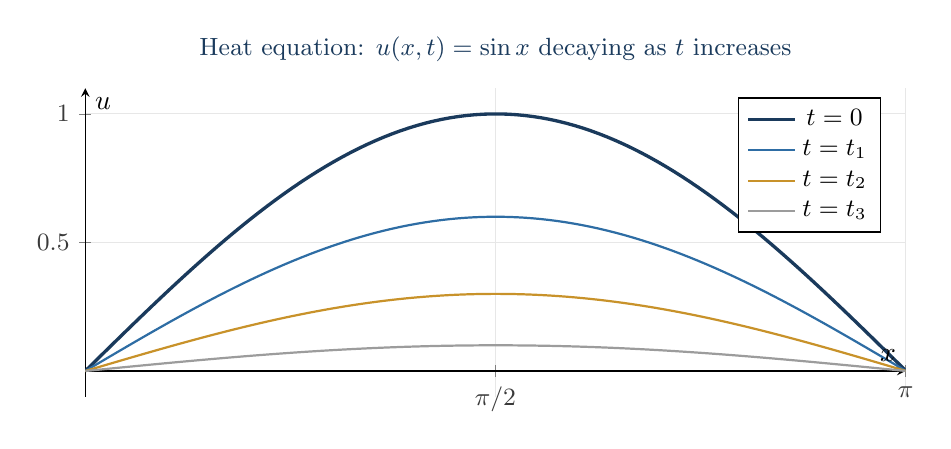
\begin{tikzpicture}
\begin{axis}[
  width=12cm,height=5.5cm,
  axis lines=center,
  xlabel={$x$},ylabel={$u$},
  xmin=0,xmax=3.14,ymin=-0.1,ymax=1.1,
  xtick={0,1.57,3.14},xticklabels={$0$,$\pi/2$,$\pi$},
  ytick={0,0.5,1},
  tick label style={font=\small,color=DarkGrey},
  grid=major,grid style={DarkGrey!12},
  title={\small\color{NavyBlue}Heat equation: $u(x,t)=\sin x$ decaying as $t$ increases},
  legend pos=north east,legend style={font=\small},
]
\addplot[NavyBlue,very thick,domain=0:3.14,samples=100]{sin(deg(x))};
\addplot[MidBlue,thick,domain=0:3.14,samples=100]{0.6*sin(deg(x))};
\addplot[Gold,thick,domain=0:3.14,samples=100]{0.3*sin(deg(x))};
\addplot[DarkGrey!50,thick,domain=0:3.14,samples=100]{0.1*sin(deg(x))};
\addlegendentry{$t=0$}
\addlegendentry{$t=t_1$}
\addlegendentry{$t=t_2$}
\addlegendentry{$t=t_3$}
\end{axis}
\end{tikzpicture}
\end{center}

\subsection{Step 3: The wave equation}

\begin{problem}
\label{prob:wave}
\begin{enumerate}[label=(\alph*),topsep=2pt]
  \item For Scenario~C, verify $u(x,y,t) = \cos(\sqrt{2}ct)\sin x\sin y$ satisfies $u_{tt}=c^2\nabla^2 u$ with the given conditions.
  \item \textbf{d'Alembert's solution} (1D wave equation $u_{tt}=c^2u_{xx}$ on $\mathbb{R}$): show the general solution is $u(x,t) = f(x-ct)+g(x+ct)$ for arbitrary $f$ and $g$. Interpret: $f(x-ct)$ is a wave moving right at speed $c$; $g(x+ct)$ moves left.
  \item With initial conditions $u(x,0)=\phi(x)$ and $u_t(x,0)=\psi(x)$: derive $u(x,t) = \frac{\phi(x-ct)+\phi(x+ct)}{2}+\frac{1}{2c}\int_{x-ct}^{x+ct}\psi(s)\,ds$.
  \item \textbf{Domain of dependence.} The value of $u(x_0,t_0)$ depends only on initial data in the interval $[x_0-ct_0, x_0+ct_0]$. Sketch the \textbf{light cone}. Why does no information propagate faster than $c$?
  \item \textbf{Standing waves} (1D with fixed endpoints). On $[0,L]$ with $u(0,t)=u(L,t)=0$: use separation to find the normal mode frequencies $\omega_n=n\pi c/L$. The general solution is a superposition of standing waves. A plucked string: if $u(x,0)=\phi(x)$ and $u_t(x,0)=0$, express the solution in terms of Fourier sine coefficients.
\end{enumerate}
\end{problem}

\begin{thought}
\textbf{d'Alembert and the nature of the wave equation.}
Jean le Rond d'Alembert derived his solution to the wave equation in 1747 by noticing that the equation factorises as $(\partial_t-c\partial_x)(\partial_t+c\partial_x)u=0$. Each factor defines a characteristic direction (slope $\pm1/c$ in the $(x,t)$-plane), and waves propagate along these characteristics. The heat equation has no characteristics in this sense --- information spreads instantaneously in all directions (the heat kernel has infinite tails). The wave equation is fundamentally different: it has a finite propagation speed, which in the context of light is the speed of light $c$. This finite speed was what forced Einstein to rethink simultaneity and give up Newtonian absolute time. The mathematics of characteristics is thus, indirectly, the origin of special relativity.
\end{thought}

\subsection{Step 4: Comparison and classification}

\begin{problem}
\label{prob:classification}
A general second-order linear PDE in two variables takes the form $Au_{xx}+2Bu_{xy}+Cu_{yy}+\cdots=0$.
\begin{enumerate}[label=(\alph*),topsep=2pt]
  \item \textbf{Classification}: the PDE is
    \begin{itemize}[noitemsep]
      \item \textbf{elliptic} if $B^2-AC<0$ (like Laplace: $1+0+1>0$, so discriminant $=0-1<0$)
      \item \textbf{parabolic} if $B^2-AC=0$ (like heat: $A=1,B=0,C=0$, discriminant $=0$)
      \item \textbf{hyperbolic} if $B^2-AC>0$ (like wave: $A=1,B=0,C=-1/c^2$)
    \end{itemize}
  Classify each of the three classical PDEs and a fourth: the Schr\"{o}dinger equation $i\hbar\partial_t\psi=-\frac{\hbar^2}{2m}\partial_x^2\psi$.
  \item Each type has qualitatively different behaviour. Elliptic equations have smooth solutions (maximum principle, no time dependence). Parabolic equations are irreversible and smooth out initial data. Hyperbolic equations propagate discontinuities along characteristics. Give one physical consequence of each type.
  \item The discriminant $B^2-AC$ is the negative of the determinant of the symbol matrix $\begin{pmatrix}A&B\\B&C\end{pmatrix}$. So elliptic equations have positive-definite symbol; hyperbolic have indefinite symbol. Connect to the classification of quadratic forms from Journey~3.
  \item \textbf{Characteristics} for a hyperbolic equation are curves in the $(x,t)$-plane along which information propagates. For the wave equation $u_{tt}=c^2u_{xx}$, find the characteristics (curves satisfying $dt/dx=\pm1/c$). Show that d'Alembert's solution is constant along each characteristic.
\end{enumerate}
\end{problem}

\begin{problem}
\label{prob:greens_pde}
\textbf{Green's functions for PDEs.}
\begin{enumerate}[label=(\alph*),topsep=2pt]
  \item The Green's function $G(\mathbf{x},\mathbf{y})$ for $-\nabla^2$ on $\mathbb{R}^3$ satisfies $-\nabla^2 G = \delta(\mathbf{x}-\mathbf{y})$. By symmetry and the fact that $\nabla^2(1/r)=0$ for $r\neq 0$ (from Module~1), show $G(\mathbf{x},\mathbf{y}) = \frac{1}{4\pi|\mathbf{x}-\mathbf{y}|}$.
  \item The Poisson equation $-\nabla^2 u = f$ has solution $u(\mathbf{x}) = \int G(\mathbf{x},\mathbf{y})f(\mathbf{y})\,d\mathbf{y} = \frac{1}{4\pi}\int\frac{f(\mathbf{y})}{|\mathbf{x}-\mathbf{y}|}\,d\mathbf{y}$. In electrostatics, this is the \textbf{Coulomb potential}: the potential due to a charge distribution $\rho$ is $\phi(\mathbf{x}) = \frac{1}{4\pi\varepsilon_0}\int\frac{\rho(\mathbf{y})}{|\mathbf{x}-\mathbf{y}|}\,d\mathbf{y}$.
  \item The \textbf{retarded Green's function} for the wave equation is $G(\mathbf{x},t;\mathbf{y},s) = \frac{\delta(t-s-|\mathbf{x}-\mathbf{y}|/c)}{4\pi|\mathbf{x}-\mathbf{y}|}$. Interpret: information from $\mathbf{y}$ at time $s$ reaches $\mathbf{x}$ at time $t=s+|\mathbf{x}-\mathbf{y}|/c$, i.e.\ exactly at light travel time.
  \item The Green's function for the heat equation is the heat kernel $G(x,t;y,s) = \frac{e^{-(x-y)^2/[4\kappa(t-s)]}}{\sqrt{4\pi\kappa(t-s)}}$ for $t>s$. Contrast with (c): heat information spreads instantaneously (the kernel is non-zero for all $x$, $t>s$), while wave information propagates at finite speed. Why is only the wave equation relativistically compatible?
\end{enumerate}
\end{problem}

\begin{problem}
\label{prob:drumhead}
\textbf{The vibrating drum.} A circular drum of radius $R$ vibrates according to $u_{tt}=c^2\nabla^2 u$ in polar coordinates, with $u(R,\theta,t)=0$ (clamped boundary).
\begin{enumerate}[label=(\alph*),topsep=2pt]
  \item Separate: try $u = R(r)\Theta(\theta)T(t)$. The angular equation gives $\Theta_n = \cos n\theta$ or $\sin n\theta$. The radial equation (with $R(R)=0$, boundedness at $r=0$) gives Bessel's equation: $R'' + \frac{1}{r}R' + \left(\lambda - \frac{n^2}{r^2}\right)R = 0$. The bounded solutions are $J_n(\sqrt{\lambda}r)$.
  \item The boundary condition $J_n(\sqrt{\lambda}R)=0$ forces $\sqrt{\lambda}R = j_{n,k}$ (the $k$-th zero of $J_n$). The normal mode frequencies are $\omega_{n,k} = cj_{n,k}/R$.
  \item The first few zeros are: $j_{0,1}\approx 2.405$, $j_{0,2}\approx 5.520$, $j_{1,1}\approx 3.832$, $j_{2,1}\approx 5.136$. Compute the ratio $\omega_{0,1}:\omega_{1,1}:\omega_{2,1}:\omega_{0,2}$. Compare with a string, where frequencies are integer multiples of the fundamental. Why does the drum sound less musical than a string?
  \item The shape of the lowest mode $u\propto J_0(j_{0,1}r/R)$ is a simple dome. The next mode $J_1(j_{1,1}r/R)\cos\theta$ has a nodal line. Sketch the nodal patterns for the first four modes. (\textbf{Chladni patterns}.)
  \item \textit{(Research.)} Mark Kac asked in 1966: ``Can you hear the shape of a drum?'' That is, does the spectrum $\{\omega_{n,k}\}$ of a drum determine its shape uniquely? In 1992 Gordon, Webb, and Wolpert found two differently-shaped drums with identical spectra. What does this say about the relationship between geometry and spectral information?
\end{enumerate}
\end{problem}

\section{Part 3 \texorpdfstring{---}{--} Discovery}

\begin{discoverybox}
\textbf{What have we built?}

\textbf{First.} The three classical PDEs --- Laplace, heat, wave --- are classified as elliptic, parabolic, and hyperbolic. This classification determines their qualitative behaviour: elliptic equations are smooth and determined by boundary values; parabolic equations are irreversible and diffuse; hyperbolic equations propagate information at finite speed.

\textbf{Second.} Separation of variables reduces a PDE to a family of ODEs. Each separated solution is a product of functions, one per variable, and the general solution is a superposition. The separation constant is an eigenvalue, and the separated solutions are eigenfunctions of the spatial operator.

\textbf{Third.} Green's functions encode the complete response of a PDE: the solution for any forcing or initial condition is a convolution (or superposition) of the Green's function with the data. The Green's function for Laplace is $1/(4\pi r)$; for the wave equation it is a delta function on the light cone; for the heat equation it is a Gaussian.

\textbf{Fourth.} The drum problem introduces Bessel functions as eigenfunctions of the Laplacian in polar coordinates, and the spectrum of the drum encodes geometric information about its shape --- but not all of it.
\end{discoverybox}

\section{Part 4 \texorpdfstring{---}{--} Naming the Ideas}

\begin{namebox}
\textbf{The three classical PDEs.}

\textbf{Laplace}: $\nabla^2 u = 0$ --- elliptic; equilibrium; smooth; maximum principle; mean value property.

\textbf{Heat}: $u_t = \kappa\nabla^2 u$ --- parabolic; diffusion; irreversible; smooths initial data; heat kernel $e^{-r^2/4\kappa t}$.

\textbf{Wave}: $u_{tt} = c^2\nabla^2 u$ --- hyperbolic; propagation; time-reversible; d'Alembert solution; characteristics; finite speed $c$.

\textbf{Classification}: $Au_{xx}+2Bu_{xy}+Cu_{yy}+\cdots$: elliptic ($B^2<AC$), parabolic ($B^2=AC$), hyperbolic ($B^2>AC$).
\end{namebox}

\section{Part 5 \texorpdfstring{---}{--} Deep Problems}

\begin{deepproblem}[The maximum principle and uniqueness]
\begin{enumerate}[label=(\alph*)]
  \item \textbf{Strong maximum principle for Laplace}: if $\nabla^2 u \leq 0$ (subharmonic) on a connected open domain $\Omega$ and $u$ attains its maximum at an interior point, then $u$ is constant. Prove the weak version: a harmonic function ($\nabla^2 u=0$) attains its maximum on $\partial\Omega$.
  \item Use the maximum principle to prove uniqueness for the Dirichlet problem ($\nabla^2 u=f$ in $\Omega$, $u=g$ on $\partial\Omega$).
  \item \textbf{For the heat equation}: if $u_t \leq \kappa\nabla^2 u$ on $[0,T]\times\Omega$ with $u\leq 0$ on the parabolic boundary (initial time and spatial boundary), then $u\leq 0$ everywhere. Use this to prove uniqueness for the heat equation with Dirichlet boundary conditions.
  \item \textbf{No maximum principle for wave equation}: give an explicit example showing that a solution to $u_{tt}=c^2u_{xx}$ can attain its maximum in the interior. Why is there no maximum principle for hyperbolic equations?
  \item The maximum principle for the heat equation implies: once a smooth initial temperature distribution begins evolving, it can never create a new local maximum in the interior. Interpret physically: is this obvious from the physics of heat conduction?
\end{enumerate}
\end{deepproblem}

\begin{deepproblem}[Fundamental solutions and distributions]
\begin{enumerate}[label=(\alph*)]
  \item The Dirac delta ``function'' $\delta(x)$ satisfies $\int_{-\infty}^\infty\delta(x)f(x)\,dx=f(0)$ for all test functions $f$. It is not a function but a \textbf{distribution} (a continuous linear functional on smooth functions). Show that $\delta'(x)$ (as a distribution) satisfies $\int\delta'(x)f(x)\,dx = -f'(0)$.
  \item The \textbf{Heaviside function} $H(x) = 0$ ($x<0$), $1$ ($x\geq 0$) satisfies $H'=\delta$ in the distributional sense. Verify: $\int H'(x)f(x)\,dx = -\int H(x)f'(x)\,dx = f(0)$.
  \item The \textbf{fundamental solution} of $-\partial_x^2$ in 1D is the function satisfying $-G''=\delta$. Find $G(x) = \frac{1}{2}|x|$ and verify. This is the 1D Green's function for the Laplacian.
  \item In $\mathbb{R}^3$, $-\nabla^2 G = \delta(\mathbf{x})$ has solution $G = \frac{1}{4\pi r}$. Show this holds: compute $-\nabla^2(1/r)$ in distribution theory by integrating against a test function and using the divergence theorem.
  \item The \textbf{Sobolev spaces} $H^s(\mathbb{R}^n)$ consist of distributions whose Fourier transform satisfies $\int(1+|\xi|^2)^s|\hat{f}(\xi)|^2<\infty$. They provide the right function spaces for PDE existence and regularity theory. State (without proof) the Sobolev embedding theorem: $H^s\subset C^k$ when $s>k+n/2$.
\end{enumerate}
\end{deepproblem}

\begin{deepproblem}[Nonlinear PDEs: shocks and solitons]
\begin{enumerate}[label=(\alph*)]
  \item The \textbf{Burgers equation} $u_t + uu_x = 0$ is a simple nonlinear wave equation. The method of characteristics: $du/dt=0$ along curves $dx/dt=u$. For initial data $u(x,0)=f(x)$, the solution is $u(x,t) = f(x-ut)$ (implicit). Find where and when characteristics cross (when do two characteristics carry different values to the same point?).
  \item At a \textbf{shock}, characteristics from different directions collide. For $f(x)=1/(1+x^2)$: show that characteristics starting from $x_0$ and $x_0+\epsilon$ meet at time $t^* = \min_x(-1/f'(x))$. Compute $t^*$.
  \item The \textbf{KdV equation} $u_t + 6uu_x + u_{xxx} = 0$ balances nonlinear steepening (from $uu_x$) with dispersion (from $u_{xxx}$). It has soliton solutions: $u(x,t) = -\frac{v}{2}\text{sech}^2\left(\frac{\sqrt{v}}{2}(x-vt)\right)$. Verify this satisfies KdV.
  \item Solitons pass through each other without changing shape. This was observed numerically by Zabusky and Kruskal in 1965 and is related to the complete integrability of KdV. Describe what ``complete integrability'' means informally.
  \item \textbf{Physical context}: solitons appear in optical fibres (pulses that don't disperse), water waves (observed by John Scott Russell in the Edinburgh canal in 1834), and Bose-Einstein condensates. What property of the medium allows a soliton to exist?
\end{enumerate}
\end{deepproblem}

\section{Part 6 \texorpdfstring{---}{--} Reflection}

\begin{reflectionbox}
\textbf{Your reflection task.}

\begin{enumerate}
  \item \textbf{On irreversibility.} The heat equation is irreversible: you cannot run it backwards. Yet it is derived from reversible molecular collisions. This is the \textbf{arrow of time} problem. Write a paragraph: where does irreversibility enter? Is it in the mathematics, in the physics, or in our description of the initial conditions?

  \item \textbf{On ``hearing the shape of a drum.''} The spectrum of a drum does not uniquely determine its shape. Yet in quantum mechanics, the energy spectrum of an atom was used to discover the structure of the atom before any direct observation was possible. Write a paragraph: what does it mean for a spectrum to determine structure, and when does it fail?

  \item \textbf{On finite vs.\ infinite propagation speed.} The heat equation predicts that heat from a match lit in Nairobi would instantaneously (if infinitesimally) affect the temperature in Tokyo. The wave equation propagates information at finite speed $c$. Which is more physically realistic? Is the heat equation ever used in relativity-compatible theories?

  \item \textbf{Looking ahead.} Module~4 studies the Schr\"{o}dinger equation: the wave equation of quantum mechanics. You have classified it as parabolic (Problem~\ref{prob:classification}). But it also has wave-like solutions. What is the difference between the quantum-mechanical wave function and a classical wave?
\end{enumerate}
\end{reflectionbox}

\medskip
\noindent\textbf{Looking ahead.}
Module~4 studies quantum mechanics as the natural continuation of the mathematics built in this module: the Schr\"{o}dinger equation, wave functions, energy levels, and the connection between PDEs, eigenvalues, and physical observables.

\vspace{1.4cm}
\begin{center}
{\color{MidBlue}\rule{0.5\linewidth}{0.8pt}}\\[6pt]
{\small\color{DarkGrey}\textit{End of Journey 4, Module 3 --- The Classical PDEs}}\\[4pt]
{\small\color{DarkGrey}Continue to: \textbf{Module 4 --- Quantum Mechanics}}\\[6pt]
{\color{MidBlue}\rule{0.5\linewidth}{0.8pt}}
\end{center}

\end{document}